\documentclass[tikz]{standalone}

\usetikzlibrary{positioning}

\usepackage{xcolor}
\definecolor{morange}{RGB}{255,127,14}
\definecolor{mblue}{RGB}{31,119,180}
\definecolor{mred}{RGB}{214,39,40}
\definecolor{mpurple}{RGB}{148,103,189}
\definecolor{mgreen}{RGB}{44,160,44}


\begin{document}

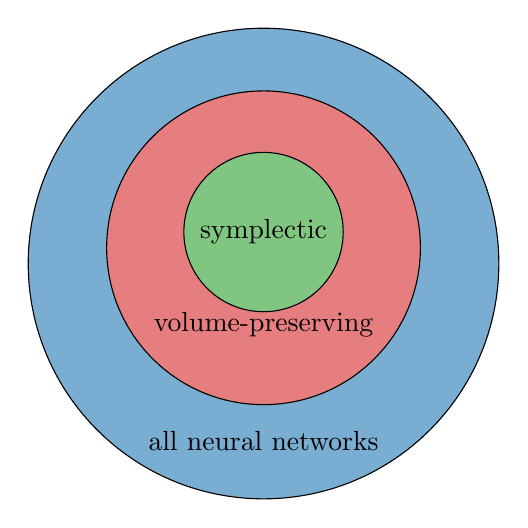
\begin{tikzpicture}[set/.style={draw,circle,inner sep=0pt,align=center}]
    \node[set,fill=mblue!60,text width=6cm,label={[below=5cm of rea,text opacity=1]all neural networks}] (nat) at (0,-0.4)  (rea) {};
    \node[set,fill=mred!60,text width=4cm,label={[below=2.7cm of int]volume-preserving}] (int) at (0,-0.2)  {};
    \node[set,fill=mgreen!60,text width=2cm] (nat) at (0,0) {symplectic};
\end{tikzpicture}

\end{document}